\section{Introduzione}

La convergenza di computer e comunicazioni ha avuto un'influenza profonda sul modo in cui sono strutturati i calcolatori. Il concetto di ``centro di calcolo'' come una stanza con un grande computer dove gli utenti portano il loro lavoro per l'elaborazione oggi è completamente superato. Il vecchio modello di un solo computer che soddisfa l'intera necessità di calcolo dell'organizzazione è stato sostituito da un altro, in cui il lavoro è svolto da un gran numero di computer distinti ma interconnessi. Questi sistemi sono chiamati \textbf{reti di calcolatori}. Due computer sono interconnessi se sono in grado di scambiare informazioni tra di loro.

\subsection{Scopi delle reti di calcolatori}

L'obiettivo della \textbf{condivisione delle risorse} è quello di rendere disponibili a chiunque sulla rete tutti i programmi, le periferiche e soprattutto i dati, indipendentemente dalla posizione fisica dell'utente e della risorsa.

Nella sua forma più semplice, ci si può immaginare il sistema informatico di un'azienda come formato da uno o più database e da un certo numero di impiegati che hanno bisogno di accedervi remotamente. In questo modello i dati sono memorizzati in computer ad alte prestazioi chiamati \textbf{server}. Al contrario gli impiegati devono poter accedere ai dati e hanno sulla loro scrivania macchine più semplici chiamate \textbf{client}. Le macchine client e server sono collegate da una \textbf{rete}. Questa configurazione è chiamata \textbf{modello client-server}.

\begin{figure}[htpb]
\centering
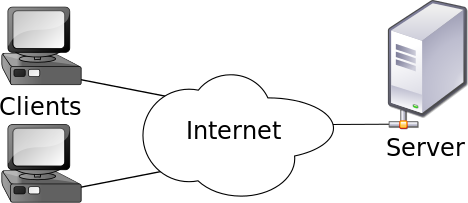
\includegraphics[scale=1]{images/client-server-model.png}
\caption{Modello client-server}
\end{figure}

